%Pacotes Primários
\documentclass[a4paper, 12pt, onecolumn]{article}   %Tipo de Documento
\usepackage[utf8]{inputenc}     %inclui todos os caracteres
\usepackage{indentfirst}        %paragrafia a primeira coluna
\usepackage[brazilian]{babel}   %Coloca o texto em português
\usepackage{setspace}%permite alterar o espaçamento entre linhas
%----------------------------------------------------------------------------------
%Pacotes secundários
\usepackage{geometry}           %definir as margens com o geometry
 \geometry{                     %Coloca As Margens
 right=2cm,                     %esquerda
 left=3cm,                      %direita
 top=3cm,                       %cima  
 bottom=2cm                     %baixo
 }
\usepackage{listings}           %trabalha com python
\usepackage[table,xcdraw]{xcolor}%cores no gráfico de python
\usepackage{multicol}           %coloca multiplas colunas
\usepackage{lipsum}             %coloca lorem ipsum
\usepackage[hidelinks]{hyperref}%Formatar URL na bibliografia
%\usepackage[nottoc]{tocbibind} %não precisa citar para aparecer na bibliografia
\usepackage{wrapfig}            %trabalha com imagens
\usepackage{cancel}             %símbolo de cancelar
\usepackage[T1]{fontenc}        %trabalha com a fonte
\usepackage{ragged2e} %trabalha com o alinhamento
\usepackage{fancyhdr}           %mexe com a paginação
\usepackage{graphicx}           %Permite colocar imagens no documento
%\usepackage[alf]{abntex2cite}
\usepackage{cite}
\pagestyle{fancy}
\fancyhf{}
\fancyheadoffset{0cm}
\renewcommand{\headrulewidth}{0pt}  %tira a linha do cabeçalho
\renewcommand{\footrulewidth}{0pt}  %tira a linha do rodapé
\fancyhead[R]{\thepage}
\fancypagestyle{plain}{
  \fancyhf{}
   \fancyhead[R]{\thepage}
}   %isso tudo faz a numeração páginas ficarem na parte superior esquerda do documento
\usepackage{amsthm,amsmath,amsfonts} %amsthm faz teoremas matemáticos, e o amsmath faz alinhamentos e expressões matemáticas, já o amsfonts disponibiliza mais funções com a fonte nas ambiente de matemática.

\usepackage{float} %permite que as imagens e tabelas possam ser posicionadas mais corretamente com o [H]

\usepackage{amssymb} %adiciona mais símbolos matemáticos
\numberwithin{table}{section}
%\numberwithin{equation}{subsection} %isso faz as equações aparecerem com a referência do respectivo capítulo
\allowdisplaybreaks %serve para permitir quebras de páginas enquanto estiver em um laço de alinhamento escrevendo uma equação
\renewcommand{\listfigurename}{List of plots}
\renewcommand{\listtablename}{Tables}
\vspace{5pt}

\bibliographystyle{plain}     % We choose the "plain" reference style

\usepackage{float}
%\usepackage[final]{listofsymbols}
\usepackage{nomencl} %para fazer lista de símbolos https://www.overleaf.com/learn/latex/Nomenclatures
\makenomenclature
\usepackage{siunitx} %para colocar as unidades

%\usepackage{etoolbox} %poder fazer grupos 

%\renewcommand\nomgroup[1]{% esse comando é caso for fazer subgrupos de símbolos
  %\item[\bfseries
  %\ifstrequal{#1}{A}{Physics Constants}{%
  %\ifstrequal{#1}{B}{Number Sets}{%
  %\ifstrequal{#1}{C}{Other Symbols}{}}}%
%]}
\newcommand{\nomunit}[1]{%
\renewcommand{\nomentryend}{\hspace*{\fill}#1}}
\setlength{\headheight}{24pt}
\usepackage{tocloft}
\newcommand{\listequationsname}{Lista de Equações}
\newlistof{myequations}{equ}{\listequationsname}
\newcommand{\myequations}[1]{%
\addcontentsline{equ}{myequations}{\protect\numberline{\theequation}#1}\par}
\setlength{\cftmyequationsnumwidth}{2.5em}% Width of equation number in List of Equations

%%%%%%%%%%%%%%%%%%%%%%%%%%%%%%% DOCUMENTO %%%%%%%%%%%%%%%%%%%%%%%%%%%%%%%%%%%

\begin{document}

%\lhead{UFMT} %Coloca texto na esquerda do cabeçalho
%\chead{Relatório de XXX} %Coloca texto no meio do cabeçalho
%Esses textos não aparecerão na capa, nem na folha de rosto porque elas possuem o \titlepage, e esse comando impede de ter cabeçalho e folha de rosto nas páginas em que eles estão
%Aqui começa a colocar os arquivos onde estão os textos do trabalho, o \input coloca um arquivo de texto tex
\titlepage

\begin{titlepage}

\begin{center}
       
        \textbf{UNIVERSIDADE FEDERAL DO MATO GROSSO}\\
       
        \textbf{FÍSICA - BACHARELADO}
       
    \vspace*{3cm}

        {BRUNO MARTINS MENDES VIEIRA}

    \vfill
        
        \large{\textbf{RESUMOS DE ELETROMAGNETISMO I}}
        
    \vfill

    \vfill
    
        INSTITUTO DE FÍSICA, UFMT\\
       
        2023
            
\end{center}


\end{titlepage}

\newpage
\thispagestyle{empty}
\listoffigures

\listoftables

%\renewcommand{\nomname}{Lista de Símbolos}

\renewcommand{\nompreamble}{A lista seguinte contem todos os símbolos que serão utilizados no relatório } 

%\nomenclature{\(c\)}{Velocidade da luz no vácuo}
%\nomunit{\SI{299792458}{\meter\per\second}}

%\printnomenclature

\newpage
\thispagestyle{empty}

    \begin{center}
        
        \doublespacing
        
        \tableofcontents
        
    \end{center}

\newpage
\rhead{\thepage}
\setlength{\parindent}{20pt}
\justifying
\section{Introdução ao Eletromagnetismo}
O eletromagnetismo é um campo de estudo que se concentra nos efeitos do campo e da radiação produzidos pelo movimento de cargas elétricas. Ele fornece uma descrição matemática e física da interação entre essas cargas, visando compreender o comportamento de uma carga elétrica quando exposta a campos elétricos e magnéticos gerados por outras cargas.

A matéria é o resultado da combinação do estudo da eletricidade com o magnetismo. Essa união se deve às descobertas feitas por Ørsted em 1820, quando ele observou que uma corrente elétrica gerava um campo magnético, e por Faraday em 1831, quando ele descobriu que um campo magnético podia induzir uma corrente elétrica. Essas descobertas foram fundamentais para o desenvolvimento do eletromagnetismo como campo de estudo.

O eletromagnetismo está inserido nos quatro principais domínios da física: mecânica clássica, mecânica quântica, relatividade e teoria de campos. Ao considerarmos que um sistema reage quando uma força é aplicada sobre ele, podemos identificar as forças fundamentais envolvidas nesse processo.



As quatro principais forças fundamentais conhecidas são:

\begin{enumerate}
    \item  Força gravitacional: é descrita pela teoria da gravitação de Albert Einstein e Isaac Newton, chamada de relatividade geral. Essa teoria descreve a interação gravitacional entre corpos massivos.

    \item Força eletromagnética: é descrita pela teoria eletromagnética de James Maxwell. Ela engloba tanto a interação elétrica quanto a interação magnética entre partículas carregadas.

    \item Força nuclear forte: é responsável pela coesão do núcleo atômico e é descrita pela teoria cromodinâmica quântica (QCD). Essa teoria descreve a interação entre quarks e glúons, que são as partículas constituintes dos hádrons.

    \item Força nuclear fraca: é responsável por processos de decaimento radioativo e é descrita pela teoria eletrofraca. Essa teoria unifica a interação fraca com a interação eletromagnética em um único formalismo.
\end{enumerate}
\newpage
Onde essas forças podem ser ranqueadas por meio de suas intensidades

\begin{table}[h]
\centering
\caption{Forças fundamentais na natureza por ordem de intensidade}
\label{tab:forcasnatureza}
\begin{tabular}{|c|c|}
\hline
\textbf{Força}  & \textbf{Intensidade}    \\ \hline
Forte           & 10                      \\ \hline
Eletromagnética & $10^{-2}$  \\ \hline
Fraca           & $10^{-13}$\\ \hline
Gravitacional   & $10^{-42}$\\ \hline
\end{tabular}
\end{table}



Todas as forças são explicadas teoricamente com base no eletromagnetismo, pois é a única teoria totalmente compreendida. Ao estudar o efeito do campo elétrico, é fundamental compreender as propriedades das cargas elétricas. As cargas elétricas podem ser classificadas em negativas e positivas. Essa distinção é baseada em observações experimentais e descreve a natureza das partículas carregadas. Por exemplo, elétrons têm carga negativa, enquanto prótons têm carga positiva.
    
A carga elétrica é sempre conservada, a menos que haja contato com uma carga oposta equivalente, por exemplo, se um objeto carregado positivamente tocar um objeto carregado negativamente, elétrons do objeto negativo podem se mover para o objeto positivo, neutralizando parte ou toda a carga positiva.  A quantidade total de cargas positivas e negativas permanece a mesma, mas sua distribuição pode ser alterada pela atração e repulsão entre as cargas. Além disso, a carga elétrica é quantizada, o que significa que ela possui um valor mínimo e não pode ser dividida infinitamente.

\newpage
\section{Cálculo Diferencial}
A derivada ordinária de uma função $f(x) = t$ representa o quanto que aquela função variou em relação a  uma variação infinitesimal de t, como entender a velocidade de uma função. Matematicamente temos que
\begin{equation}
    dv = \frac{dx}{dt} .
\end{equation}



A derivada parcial é a derivada para uma função com duas ou mais variáveis. Neste caso há de se derivar a função em relação a uma das variáveis e manter as outras constantes. Então a função $z = f(x,y)=x^2 + 2y^3$ terá como derivada parcial em $x$ 
\begin{equation}
    \frac{\partial z}{\partial x} = 2x .
\end{equation}
O operador \textit{del} $\nabla$ (conhecido como Nabla) é importante para a construção do gradiente, divergente e rotacional, e é escrito da seguinte maneira para um sistema de três coordenadas: 

\begin{equation}
    \nabla \Vec{V} = \frac{\partial}{\partial x} \hat{\textbf{x}} + \frac{\partial}{\partial y} \hat{\textbf{y}}+\frac{\partial}{\partial z} \hat{\textbf{z}}.
\end{equation}

O Nabla é um operador mas tem uma flecha em cima, isso acontece porque ele é um operador vetorial, então ele sozinho não tem significado, mas ao colocar com uma função terá um significado.

Em uma função com várias variáveis podemos fazer algumas operações usando as derivadas parciais. O gradiente de uma função vai mostrar como que a mesma vai funcionar quando uma das variáveis seja alterada. 
O Gradiente de uma função que contém as derivadas parciais formando um vetor ao aplicar em um campo escalar. Então em uma função $f(x,y,z) = x^2 + 2xy^2 + 3z$, o seu gradiente será:

\begin{equation}
    \nabla F = 2x \hat{\textbf{x}} + 4y \hat{\textbf{y}} + 3 \hat{\textbf{z}} .
\end{equation}

O gradiente tem direção (onde terá a maior velocidade), magnitude (inclinação da reta naquela direção) e sentido (para onde aponta). Quando o gradiente foi igual a zero teremos um ponto crítico, ou no caso de uma montanha (exercício $1.12$ do Griffiths), o topo será quando igualarmos o gradiente a zero. 


O divergente é um campo escalar multiplicado pelo operador \textit{del} 

\begin{equation*}
    \nabla \cdot \textbf{v} = (\hat{\textbf{x}} \frac{\partial}{\partial x} + \hat{\hat{\textbf{y}}} \frac{\partial}{\partial y} + \hat{\hat{\textbf{z}}} \frac{\partial}{\partial z}) \cdot (v_{x} {\hat{\textbf{x}}} + v_{y} {\hat{\textbf{y}}} + v_{z} {\hat{\textbf{z}}}) ,
\end{equation*}


\begin{equation} \label{divergente}
    \nabla \cdot \textbf{v} = \frac{\partial v_{x}}{\partial x} + \frac{\partial v_{y}}{\partial y} + \frac{\partial v_{z}}{\partial z} ,
\end{equation}
\myequations{Divergente de um campo escalar}

e vai indicar o quanto que o vetor vai estar divergindo do ponto em questão. 

Se \ref{divergente} é igual a $0$ então não há divergência,  se \ref{divergente} for menor do que zero então o campo tende a ficar mais denso dentro do ponto em questão, caso \ref{divergente} seja positivo então há menos densidade naquele ponto do campo. Esta ideia pode ser entendida como uma torneira, onde

\begin{itemize}
    \item Torneira aberta: Divergente $ > 0$;
    \item Torneira fechada: Divergente $= 0$.
\end{itemize}

Em um caso hipotético onde a água entre na torneira o divergente seria $< 0$. 

O rotacional é uma função vetorial dado por um campo vetorial multiplicado por \textit{del}: 
A matriz contendo as derivadas parciais em relação às coordenadas $x$, $y$ e $z$, juntamente com os versores $\hat{x}$, $\hat{y}$ e $\hat{z}$, é dada por:
\begin{equation*}
\nabla \times  V = 
\begin{bmatrix}
{\hat{\textbf{x}}} & {\hat{\textbf{y}}} & {\hat{\textbf{z}}} \\
\frac{\partial}{\partial x} & \frac{\partial}{\partial y} & \frac{\partial}{\partial z} \\
v_{x} & v_{y} & v_{z}

\end{bmatrix}
\end{equation*}

\begin{equation}
    \nabla \times  V = \hat{\textbf{x}} \left(\frac{\partial v_{z}}{\partial y} - \frac{\partial v_{y}}{\partial z }\right) + \hat{\textbf{y}} \left(\frac{\partial v_x}{\partial z } - \frac{\partial v_{z}}{\partial x}\right) + \hat{\textbf{z}} \left(\frac{\partial v_{y}}{\partial x} - \frac{\partial v_{x}}{\partial y}\right) . 
\end{equation}
\myequations{Rotacional de um campo vetorial}

Essa função vai medir o quanto que o vetor rotaciona em relação a um ponto em discussão, impactando um vetor tridimensional próxima que irá rotacionar e assim sucessivamente. 

\newpage\section{Eletrostática}
O estudo de cargas estacionárias é chamado de \textbf{Eletrostática}. Uma carga estacionária no espaço consegue produzir um \textbf{campo elétrico}. Um campo pode ser definido como uma região no espaço onde em cada posição há uma característica distinta, sendo importante para compreender um fenômeno, sendo descrito com direção, sentido e módulo. 

O campo elétrico pode ser demonstrada com a \textbf{Lei de Coulomb}, que diz que a força entre duas partículas aumenta quando a carga aumenta e decai com o inverso do quadrado da distância (quanto mais longe menor a força). É escrita da seguinte maneira:

\begin{equation} \label{coulumb}
    \Vec{F} = \epsilon_{0} \frac{{q_{1}}{q_{2}}}{d^2} \hat{\textbf{r}},
\end{equation}
\myequations{Lei de Coulumb}



onde $q_{1}$ e $q_{2}$ são as cargas de teste, $d$ é a distância entre as partículas, $\hat{\textbf{r}}$ é o vetor separação e $k_{0}$ é a constante de Coulomb, sendo dada pela relação
 
\begin{equation*}
    \epsilon_{0}= \frac{1}{4 \pi \epsilon_{0}},
\end{equation*}

e tem o valor de $8.988 \times 10^9 N\times M^2 \times C^{-2}$.

O principal problema que o eletromagnetismo tenta resolver é qual a força que um conjunto cargas consegue exercer sobre outras cargas e para isto existe o \textbf{princípio de superposição}. Este princípio diz que uma carga consegue exercer uma força de maneira individual sobre outra carga e que, em um cenário onde haja uma carga de teste $Q_{1}$ com ene cargas ao seu redor, a força exercida sobre a carga $Q_{1}$ será a soma da força de cada uma das cargas, como se todas as cargas fossem juntadas em uma única carga $Q$. Matematicamente temos o seguinte:

\begin{equation} \label{superposicao}
    \vec{F}_{Q \rightarrow Q_{1}} = \vec{F}_{1} + \vec{F}_{2} + \vec{F}_{3}+...+\vec{F}_{n}.
\end{equation}

Utilizando a equação \ref{coulumb} podemos escrever equação \ref{superposicao} como:

\begin{equation*}
    \vec{F}_{Q \rightarrow Q_{1}} = \vec{F}_{1} + \vec{F}_{2} + ... + \vec{F}_{n} = \epsilon_{0}\left(\frac{q_{1}Q_{1}}{r_{1}^2} + \frac{q_{2}Q_{1}}{r_{2}^2} + \frac{q_{3}Q_{1}}{r_{3}^2} + ... + \frac{q_{n}Q_{1}}{r_{n}^2}\right) 
\end{equation*}
\myequations{Princípio da Superposição}

\begin{equation}
    \vec{F} = Q\Vec{E},
\end{equation}

onde $\vec{E}$ é a soma dos campos de todas as cargas fontes.


%Um campo elétrico pode ser visualizado utilizando as linhas de campo, como na figura a seguir

As linhas de campo elétrico são desenhadas de tal forma que em cada ponto, a direção da linha indica a direção do campo elétrico local e a densidade das linhas está relacionada à intensidade do campo elétrico. Em outras palavras, as linhas de campo elétrico são mais densas em regiões onde o campo elétrico é mais intenso e mais esparsas onde o campo elétrico é mais fraco.

As linhas de campo elétrico começam nas cargas positivas e terminam nas cargas negativas. Isso ocorre porque as cargas positivas emitem linhas de campo elétrico que se afastam delas, enquanto as cargas negativas emitem linhas de campo elétrico que se aproximam delas.

As linhas de campo elétrico nunca se cruzam, o que significa que em cada ponto do espaço, apenas uma direção e intensidade do campo elétrico são válidas. Se as linhas de campo elétrico se cruzassem, isso implicaria em um ponto o campo ter dois valores.

Com a ideia de linhas de campo podemos construir o conceito de fluxo de campo elétrico, que pode ser definido como \textit{a quantidade de linhas de campo que passam através de uma superfície}. Logo o fluxo é diretamente proporcional as linhas de campo e pode ser definido como

\[\phi_{E} \equiv \int_{S} E \cdot d\textbf{a} .\] \myequations{Fluxo do campo elétrico}

O fluxo dentro de uma superfície fechada será o indicativo da carga líquida que há em seu interior, com isso, uma carga externa não consegue interferir no fluxo de uma superfície $S$. Isso é a base da \textbf{lei de Gauss}.  O fluxo dentro de uma esfera com uma carga será


\[\oint E \cdot d\textbf{a} = \int \frac{1}{4 \pi \epsilon_{0}} (\frac{q}{r^2}\hat{\textbf{r}})\cdot (r^2 sin \theta d\theta d\phi \hat{\textbf{r}}) = \frac{q}{\epsilon_{0}}.\] 
O mesmo princípio de superposição utilizado no inicio serve para quando houver mais de uma carga dentro da esfera, então


\[\oint E \cdot d\textbf{a} = \sum_{i=1}^n (\frac{q_{i}}{\epsilon_{0}}). \]

O \textbf{potencial elétrico} é uma maneira simplificada de representar o campo elétrico. Toda carga elétrica gera um campo elétrico que, quando colocarmos uma carga de teste $q$ terá uma pode ser definido como


\[ V(r) \equiv - \int_{O}^r \textbf{E} \cdot d\textbf{l}, \] \myequations{Potencial Elétrico}
onde $O$ é um ponto de referência arbítrio. Por ser arbitrária o potencial não é uma grandeza física, já que para cada ponto de referência haverá um valor de potencial diferente, com isso o único resultado que de fato importa é a diferença de potencial entre dois pontos. Usualmente se escolhe o infinito como ponto de referência, já que ali o potencial vale zero. 

A diferença entre os pontos $a$ e $b$ vai resultar no seguinte potencial.


\[ V(r) = - \int_{a}^{b} \textbf{E} \cdot d\textbf{l}.\]

Com o teorema fundamental dos gradientes temos que


\[\int_{a}^{b} (\nabla V) \cdot d\textbf{l} = - \int_{a}^{b} \textbf{E} \cdot d\textbf{l},\]

logo 


\[E = - \nabla V\]
significando que quando fazemos o gradiente do potencial encontramos o campo elétrico. 


\newpage\section{Continuidade e Descontinuidade}Em uma situação onde temos uma superfície $S$ onde há uma densidade de carga $\sigma$  e um campo elétrico $\Vec{E}$ que está perpendicular a superfície $S$. Nesse caso fica a questão de saber se o campo elétrico $\Vec{E}$ será o mesmo ao atravessar a superfície $S$. 
Primeiramente podemos utilizar a lei de Gauss, onde 
\begin{equation}
    \oint \Vec{E}_{tot} \cdot d\mathbf{a} = \frac{Q_{enc}}{\epsilon_{0}} = \frac{\sigma A}{\epsilon_{0}},
\end{equation}
onde $A$ é a área da superfície gaussiana. Como $E_{tot}$ é o campo elétrico total, então 

\begin{equation}
    \left(\oint \Vec{E}_{acima} da\right) \cdot \hat{n} +\left(\oint \Vec{E}_{abaixo} da\right) \cdot\hat{n} = \frac{\sigma A}{\epsilon_{0}}
\end{equation}
como o vetor normal $\hat{n}$ é um vetor que sai da superfície, então o vetor normal do campo elétrico abaixo será o oposto do campo acima - já que estão em direção oposta - com isso
\begin{equation*}
    \left(\oint\Vec{E}_{acima} \cdot da -\oint \Vec{E}_{abaixo} \cdot da\right) \cdot \hat{n} = \frac{\sigma A}{\epsilon_{0}},
\end{equation*}
resultando em 

\begin{equation}
    \Vec{E}_{acima} - \Vec{E}_{abaixo} = \frac{\sigma}{\epsilon_{0}}.
\end{equation}
\myequations{Equação da descontinuidade do campo elétrico}
Com esse resultado vemos que quando o campo for perpendicular ao passar pela superfície S, o campo elétrico \(\Vec{E}_{acima}\) será diferente do campo elétrico abaixo \(\Vec{E}_{abaixo}\), isto é, ele será  \textbf{descontínuo} com um fator $\sigma/\epsilon_0$. 


   % 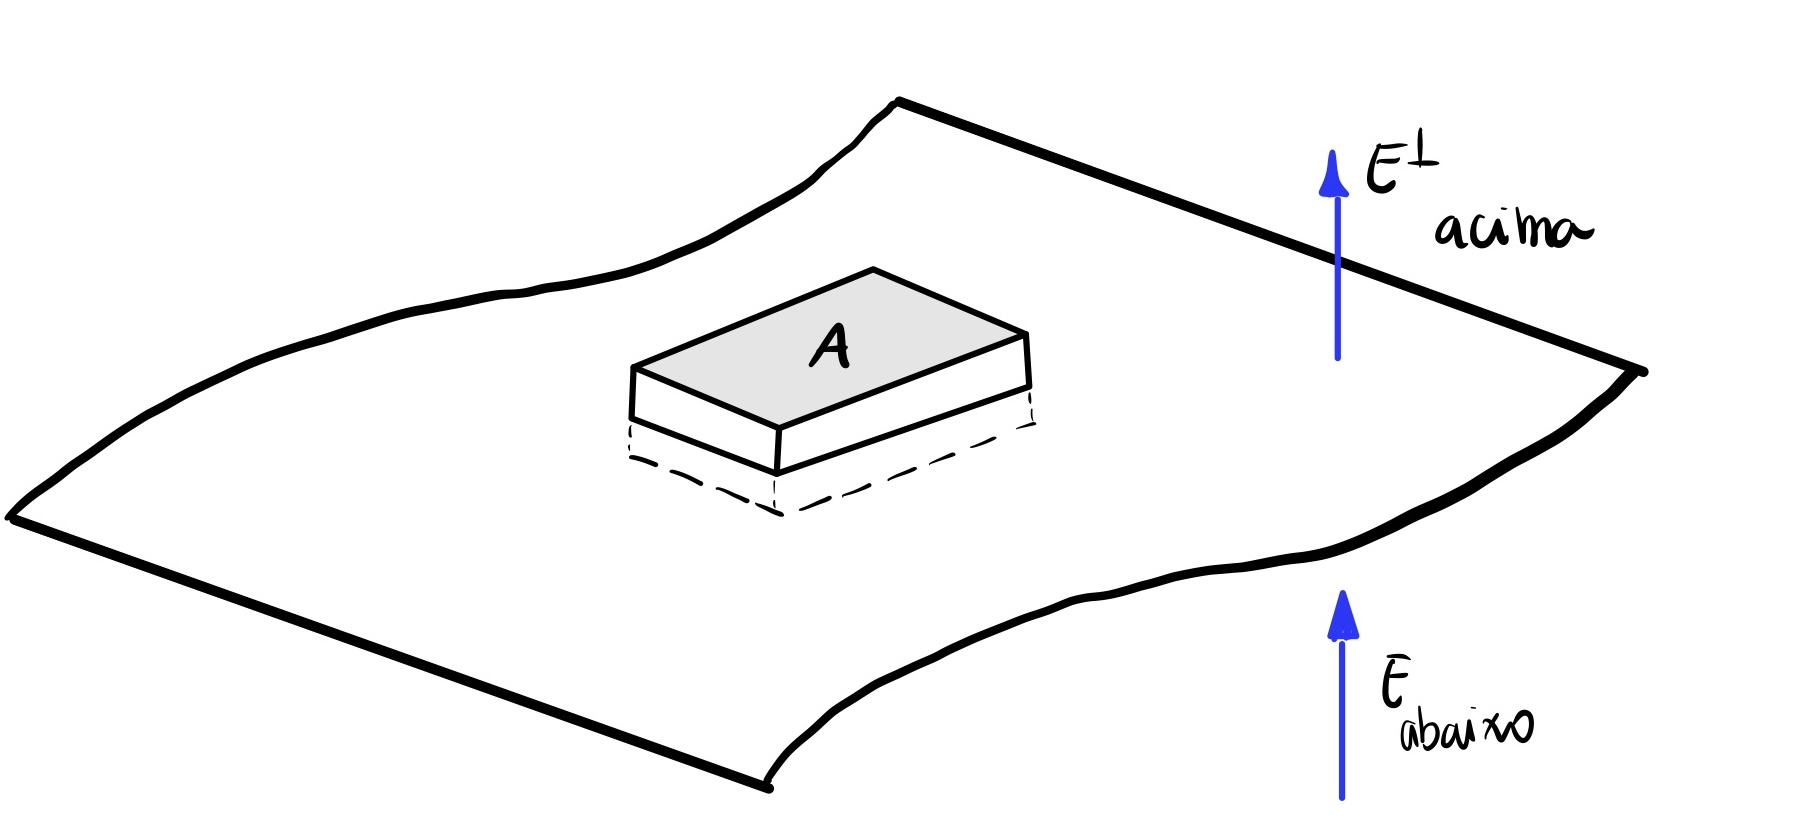
\includegraphics[width=0.5\linewidth]{IMG_3012.jpeg}
    

Agora quando o campo elétrico está tangente ao campo elétrico não haverá \textbf{descontinuidade}, porque as linhas de campo serão ortogonais, então o produto escalar entre eles dará que o ângulo do cosseno será igual a zero.  Com isso teremos que

\begin{equation}\label{seila}
    \Vec{E}_{acima} - \Vec{E}_{abaixo} = \frac{\sigma}{\epsilon_{0}} \hat{\vec{n}}
\end{equation}
\(\hat{n}\) será igual a $0$ (zero), consequentemente 


\[\Vec{E}_{acima} - \Vec{E}_{abaixo} = \frac{\sigma}{\epsilon_{0}} \cdot 0 \xrightarrow{}\Vec{E}_{acima} = \Vec{E}_{abaixo}\]




%\begin{figure}[h]
    %\centering
    %\caption{Campo elétrico tangente a superfície}
    %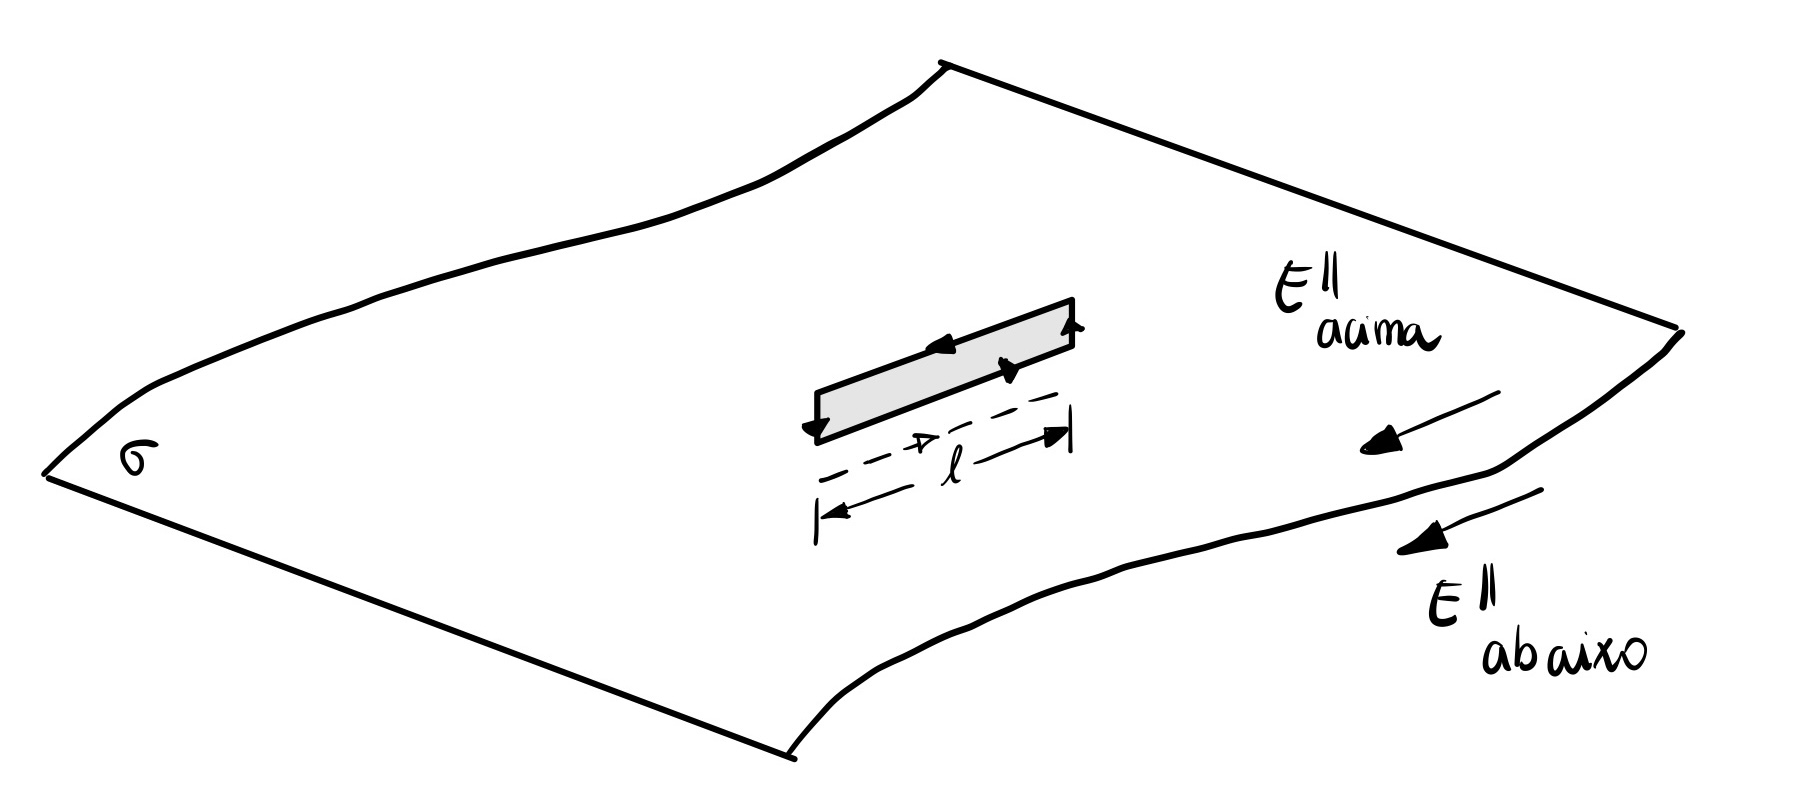
\includegraphics[width=0.5\linewidth]{IMG_3013.jpeg}
    
 %   \label{fig:enter-label}
%\end{figure}


O \textbf{potencial} entre dois pontos é dado por

\[V(b)-V(a) = - \int_{O}^{b} E\cdot d\textbf{l} +\int_{O}^{a} E\cdot d\textbf{l} \]
\[V(b)-V(a) = - \int_{a}^{b} E\cdot d\textbf{l}.\]
Quando há uma superfície entre os pontos temos


\[V_{acima} - V_{abaixo} = - \int_{a}^{b} E \cdot d\textbf{l},\]
conforme a distância entre os pontos $a$ e $b$ vai diminuindo, ficando próxima a espessura da superfície, a integral tende a zero, logo 


\[V_{acima} = V_{abaixo},\]
isto é, não há descontinuidade. Mas quando aplicamos o divergente na equação \ref{seila} (já que \(E = -\nabla V\)) temos que
\[\nabla V_{acima}-\nabla V_{abaixo} = -\frac{\sigma}{\epsilon_{0}} \hat{\textbf{n}}\]
implicando que por mais que o potencial não tenha descontinuidade o gradiente dele terá. Como o campo elétrico $E$ é igual a menos o gradiente do potencial então poderia - eu suponho - que dá para afirmar que caso o campo seja descontinuo o negativo do gradiente do potencial também será descontinuo, sem fazer conta alguma. 
\newpage\section{Teorema da Unicidade}Como o objetivo é encontrar o campo elétrico, poderíamos resolver pela lei de Coulomb, mas nem sempre será fácil resolver essa integral, por mais que em alguns momentos podemos utilizar simetria facilitando a resolução. Mesmo com o potencial $\Vec{V}$ pode ser complicado resolver a integral e depois encontrar o gradiente. 

Para resolver esse impasse utilizamos técnicas especiais. Utilizando equação de Poisson 
\[\nabla ^2 V = -\frac{\rho}{\epsilon_{0}}\]
poderíamos encontrar o campo elétrico, onde a solução dessa equação é o potencial. Utilizando algumas condições de contorno conseguiríamos resolver sem problema algum. Usando \(\rho = 0\), um local onde é um espaço vazio com cargas longes que estão criando um potencial, reduzimos a equação a 
\[\nabla^2 V=0,\]
ou em coordenadas cartesianas 
\[\frac{\nabla^2 V}{\partial x^2} + \frac{\nabla^2 V}{\partial y^2} + \frac{\nabla^2 V}{\partial z^2}=0. \]
 Para uma  dimensão a equação tem como solução 
\[ V(x) = mx +b,\]
mas a partir de duas dimensões, não tem mais uma única solução. Como a equação se torna uma derivada parcial, há somente uma solução geral, que para encontrar é necessário dar  condições de contorno para encontrar a solução. Condições de contorno são são especificações adicionais fornecidas para determinar uma solução única para a equação. A escolha adequada das condições de contorno é crucial para garantir que o problema tenha uma solução única e bem-definida. Se a solução for encontrada satisfazendo as condições de contorno e a equação de Laplace, logo a solução é única.  
Um conjunto de condições de contorno forma um \textbf{teorema de unicidade}. Há dois teoremas que são mais úteis: 
\begin{enumerate}
    \item O primeiro diz que o potencial $V$ é determinado se for especificado na superfície de contorno, em outras palavras, se conhecemos o potencial $V$ em toda a superfície de contorno S que envolve o volume $\nu$, juntamente com a equação de Laplace sendo satisfeita dentro do volume $\nu$, então não pode haver mais de uma solução para o potencial $V$ em um volume $\nu$ que satisfaça todas essas condições.
    \item O segundo diz em um volume V cercado por condutores e contendo uma densidade de carga especificada p, o campo elétrico é determinado univocamente se a carga total de cada condutor for dada - isto é - se todas as condições de contorno forem satisfeitas e as informações sobre a carga total de cada condutor forem fornecidas, então o campo elétrico dentro do volume V será determinado de forma única. Não haverá mais de uma solução possível para o campo elétrico nesse cenário específico.
\end{enumerate}
\input{Secoes/6_métodos das imagens}
\newpage\section{Polarização}
Na natureza temos dois tipos de materiais:
\begin{enumerate}
    \item \textbf{Condutores}:  São materiais que possuem a capacidade de permitir o fluxo de corrente elétrica com relativa facilidade. Isso ocorre porque os elétrons em um condutor estão fracamente ligados aos seus átomos, permitindo que eles se movam livremente sob a influência de uma diferença de potencial elétrico.
    \item \textbf{Isolantes} (dielétricos): São materiais que não conduzem eletricidade facilmente. Quando um campo elétrico é aplicado a um dielétrico, os elétrons não podem se movimentar livremente através dele, como ocorre em um condutor. Isso acontece devido à forte ligação dos elétrons em um dielétrico aos seus átomos, impedindo o fluxo de corrente elétrica.
\end{enumerate}

Ao aplicarmos um campo elétrico $\vec{E}$ a um condutor, as partículas se movem sem impedimento. No entanto, quando aplicamos o mesmo campo a um dielétrico, ocorre uma redistribuição das cargas. O núcleo se desloca em direção ao campo elétrico, enquanto os elétrons se movem em direção oposta, criando um dipolo de polarização $\vec{p}$. Esse dipolo é diretamente proporcional ao campo elétrico aplicado. Se o campo $\vec{E}$ for excessivamente intenso, o isolante pode se tornar ionizado.

No caso das moléculas, nem sempre ocorre o mesmo efeito, uma vez que moléculas polares são aquelas em que os elétrons estão distribuídos de maneira assimétrica, resultando em uma carga positiva parcial em uma extremidade da molécula e uma carga negativa parcial na outra extremidade. Esse desequilíbrio de cargas cria um dipolo elétrico na molécula, com uma separação de carga.

Quando um campo elétrico externo é aplicado a um material que contém moléculas polares, essas moléculas tendem a se alinhar na direção do campo. Esse alinhamento é conhecido como polarização. O campo elétrico externo exerce forças sobre as cargas parciais nas moléculas polares, fazendo com que elas girem ou se orientem de acordo com a direção do campo.


\newpage\section{ Deslocamento Elétrico}

O deslocamento elétrico é um conceito central em Eletromagnetismo. Ele descreve a densidade de carga elétrica livre  -  que é a única carga que nós conseguimos controlar - em um dado ponto de um material dielétrico. Quando aplicamos um campo elétrico externo a um material dielétrico, os elétrons das átomos deslocam-se parcialmente de suas posições de equilíbrio, criando uma polarização elétrica, ou seja, produzir acúmulos de carga ligada dentro do e na superfície do dielétrico. O deslocamento elétrico ($D$) é a soma do campo elétrico aplicado ($E$) e da polarização elétrica ($P$), onde
\begin{equation}
\vec{D} = \varepsilon_0 \vec{E} + \vec{P},
\end{equation}

onde $\varepsilon_0$ é a permissividade elétrica do vácuo. Como todas as equações de Maxwell são escritas em termos de fontes livres, então $\vec{D}$ na lei de Gauss se torna

\begin{equation}
    \nabla \cdot \vec{D} = \rho_l .
\end{equation}


\subsection{Dielétricos Lineares}

Dielétricos Lineares são caracterizados por não conduzirem corrente elétrica significativa, mas respondem de maneira linear quando expostos a um campo elétrico externo. À medida que o campo elétrico aumenta, a polarização elétrica do material também aumenta de forma proporcional. Essa relação é expressa por meio da susceptibilidade elétrica ($\chi_e$), uma constante do material que quantifica a capacidade do material de se polarizar sob a influência do campo elétrico.

A equação que descreve a relação entre o campo elétrico ($\vec{E}$), a polarização ($\vec{P}$) e a susceptibilidade elétrica é:
\begin{equation}
    \vec{P}=\epsilon_0 \chi_e \vec{E}, 
\end{equation}


onde $\varepsilon_0$ representa a permissividade elétrica do vácuo.

Quando um dielétrico linear é inserido em um campo elétrico, ele aumenta o deslocamento elétrico ($\vec{D}$) em relação ao campo aplicado ($\vec{E}$) devido à contribuição da polarização do material. Isso significa que o dielétrico efetivamente aumenta a capacidade de armazenamento de carga e energia elétrica, sendo amplamente utilizado em capacitores.

\subsection{ Energia em Sistemas Dielétricos}
Quando um dielétrico é inserido em um capacitor, a energia armazenada no capacitor aumenta devido ao aumento da capacitância resultante do dielétrico. A energia armazenada ($\vec{W}$) em um capacitor com dielétrico é dada pela fórmula
\begin{equation}
   \vec{W} = \frac{CV^2}{2},
\end{equation}
onde $C$ é a capacitância do capacitor e $V$ é a diferença de potencial entre as placas do capacitor.

Quando um capacitor é preenchido com um dielétrico linear, a capacitância é maior do que no vácuo. Isso significa que o capacitor pode armazenar uma quantidade maior de carga elétrica para o mesmo potencial elétrico aplicado. Portanto, a energia armazenada em um sistema dielétrico é maior devido à maior capacidade de armazenamento de carga, mantendo o mesmo potencial elétrico.
\newpage




\newpage\section{Magnetostática}
Até agora sabíamos que uma carga estática gerava campo elétrico, mas não sabíamos sobre cargas em movimento. As cargas em movimento geram os \textbf{campos magnéticos} e lhe é atribuído a letra $\vec{B}$. 

Um campo magnético $\vec{B}$ é capaz de exercer uma força, conhecida como \textbf{força magnética} $(\vec{F}_{mag})$ que é a força exercida por um campo magnético em um objeto ou partícula carregada magneticamente que está em movimento. Essa força atua perpendicularmente à direção do movimento e à direção do campo magnético.

A força magnética é descrita pela Lei de Lorentz, que estabelece que a força magnética ($ \vec{F}_{mag}$) em uma partícula carregada ($q$) em movimento com velocidade ($\vec{v}$) em um campo magnético ($\vec{B}$) é dada pela fórmula:

\begin{equation} \label{fmag}
    \vec{F}_{mag} = q  (\vec{v} \times\vec{B}),
\end{equation}

    onde a direção dessa força pode ser encontrada utilizando a regra da mão direita.

Uma particularidade da equação \ref{fmag} é de que a força magnética $\vec{B}$ não realiza trabalho $dW_{mag}$ sobre cargas. O trabalho realizado é calculado multiplicando a componente $\vec{F}_{mag}$ pelo deslocamento $d\mathbf{l}$. Matematicamente, o trabalho infinitesimal ($dW$) realizado pela força magnética em um deslocamento dado por um vetor deslocamento ($d\mathbf{l} = \vec{v} \textit{dt}$) é dado por:

\begin{equation}
    dW_{mag} = F_{mag} \cdot d\textbf{l} = Q(\vec{v} \times \vec{B}) \cdot \vec{v} dt,
\end{equation}

mas o vetor $\Vec{v} \times \vec{B}$ sempre terá um ângulo de 90°$(\pi / 2)$ em relação ao vetor velocidade $\vec{v}$, com isso o produto escalar entre os dois vetores $(|A||B| \cos \theta)$ resultará em zero $(\cos \pi /2 = 0)$. Então o trabalho realizado por força magnética $dW_{mag}$ será:
\begin{equation}
    dW_{mag} = 0.
\end{equation}
\newpage
\newpage\section{Magnetização e Materiais Magnéticos}A magnetização é um fenômeno em que um material adquire propriedades magnéticas devido à interação de seus átomos com um campo magnético externo. Quando um material é exposto a um campo magnético, seus dipolos magnéticos tendem a se alinhar em direção do campo aplicado, resultando na criação de um campo magnético líquido no material.

A magnetização pode ocorrer em diferentes materiais, e o resultado depende da orientação dos dipolos magnéticos em relação ao campo magnético. Esses resultados são observados em três categorias principais de materiais: \textbf{paramagnéticos}, \textbf{diamagnéticos} e \textbf{ferromagnéticos}.



Nos materiais \textbf{paramagnéticos}, os momentos magnéticos dos átomos se alinham \textit{paralelamente} com o campo magnético externo. Quando o campo magnético \textbf{$\vec{B}$} é removido, os momentos magnéticos retornam à sua orientação aleatória original. 

Os materiais \textbf{diamagnéticos} possuem momentos magnéticos \textit{opostos} ao campo magnético aplicado e também perdem quando o campo magnético \textbf{$\vec{B}$} é removido. 

Já materiais \textbf{ferromagnéticos} tem os seus dipolos magnéticos apontado paralelamente ao campo magnético \textbf{$\vec{B}$}. O que os diferencia dos outros materiais é a capacidade de reter a direção do dipolo magnético mesmo após o campo magnético ser removido. Isso os torna muito úteis para estudos e aplicações práticas, permitindo a criação de ímãs permanentes e a exploração de diversos fenômenos magnéticos.


\newpage\section{Ferromagnetismo}O \textbf{ferromagnetismo} é um fenômeno magnético em que certos materiais, como ferro,  se magnetizam de forma permanente e retem o seu magnetismo mesmo após a retirada deste campo magnético.

Uma característica distintiva do ferromagnetismo é a presença de domínios magnéticos em um material ferromagnético. Os domínios são regiões microscópicas no material onde os momentos magnéticos dos átomos estão alinhados em uma mesma direção. Cada domínio atua como um pequeno ímã, contribuindo para a magnetização total do material.


Em um material não magnetizado, os domínios magnéticos estão distribuídos aleatoriamente, resultando em um cancelamento das forças magnéticas entre eles. Portanto, a magnetização total do material é próxima de zero.

No entanto, quando um campo magnético externo é aplicado ao material ferromagnético, os domínios tendem a se alinhar com a direção do campo. À medida que o campo magnético se fortalece, os domínios se alinham cada vez mais, aumentando a magnetização total do material.

Quando o campo magnético é removido, alguns dos domínios podem permanecer alinhados, mantendo a magnetização do material. Essa propriedade é conhecida como remanência. No entanto, a magnetização remanescente pode ser reduzida ou eliminada por meio de forças externas, como aquecimento intenso ou aplicação de campos magnéticos opostos. Se o campo magnético externo for variado, obtemos o que é chamado de \textbf{ciclo de histerese}. Esse ciclo descreve o comportamento da magnetização de um material ferromagnético à medida que o campo magnético externo é variado.

Ao aumentar gradualmente a intensidade do campo magnético aplicado a um material ferromagnético a partir de zero, a magnetização do material aumenta. No entanto, a relação entre a intensidade do campo magnético aplicado e a magnetização não é linear. Em vez disso, ela exibe uma relação não linear e complexa.

Durante o aumento do campo magnético, o material passa por um ponto conhecido como ponto de saturação. Nesse ponto, a magnetização atinge seu valor máximo e não pode mais aumentar, mesmo que o campo magnético seja aumentado ainda mais. A partir desse ponto, o material está completamente magnetizado.

Agora, se começarmos a reduzir gradualmente a intensidade do campo magnético externo, o material não retorna à sua magnetização original. Isso ocorre porque o material possui uma propriedade chamada coercividade, que é a resistência do material a ter sua magnetização revertida. Para reverter a magnetização, é necessário aplicar um campo magnético oposto, com intensidade suficiente para superar a coercividade do material.

O processo de redução do campo magnético até o ponto em que a magnetização do material se torna zero é chamado de ciclo de desmagnetização. Nesse ponto, o material retorna ao estado não magnetizado.

Agora, se continuarmos a aumentar novamente a intensidade do campo magnético, observaremos um comportamento interessante. O material não segue a mesma curva de magnetização do primeiro ciclo, mas segue uma curva de magnetização diferente. Essa diferença ocorre porque o material apresenta uma memória magnética. Os domínios magnéticos que não foram completamente desfeitos durante o ciclo de desmagnetização influenciam a resposta magnética do material durante o ciclo subsequente. Essa memória resulta na formação de um novo conjunto de domínios magnéticos durante o processo de remagnetização.

O ciclo completo de magnetização, desmagnetização e remagnetização de um material ferromagnético é conhecido como \textbf{ciclo de histerese magnética.} Esse fenômeno é frequentemente representado graficamente em um gráfico que mostra a magnetização em função do campo magnético aplicado. O ciclo de histerese mostra a diferença entre a magnetização do material quando o campo magnético está aumentando e quando está diminuindo.


    %\includegraphics[width=0.5\textwidth]{Screenshot 2023-05-14 190347.png} 


A temperatura também desempenha um papel importante no ferromagnetismo. Acima de uma determinada temperatura crítica, conhecida como \textbf{temperatura de Curie}, o material ferromagnético perde suas propriedades magnéticas. Nesse ponto, a energia térmica é suficiente para perturbar a ordem dos domínios magnéticos, causando sua desorganização e redução da magnetização. Abaixo da temperatura de Curie, o material recupera suas propriedades ferromagnéticas.


\newpage\section{Lei de Faraday-Lenz e Indutância}Faraday fez uma série de experimentos que consistia em uma espira em um campo magnético $\vec{B}$ e que:

\begin{enumerate}
    \item[(a)] ao movimentar a espira;
    \item[(b)] movimentar o campo;
    \item[(c)]variar o campo magnético $\vec{B}$.
\end{enumerate}
todos os casos levavam a geração de uma corrente induzida. Isso é algo estranho porque até o momento somente campos magnéticos que geravam corrente e, no segundo caso, a espira esta parada. Isso levou  Faraday a concluir que o que gerava a corrente era os campos elétricos.


    %\includegraphics[scale=0.6]{induçãoeletromagnetica.jpg}


Com isso ele propôs que
\begin{quote}
\begin{center}
   \boxed{ \textit{Um campo magnético que varia induz um campo elétrico}}
\end{center}
\end{quote}

onde matematicamente é dado pela equação
\begin{equation} \label{eq1}
    {\vec{\nabla} \times \vec{E} = \frac{\partial \vec{B}}{\partial t},}
\end{equation}

que é conhecida como \textbf{lei de Faraday}. Se caso o campo for constante então o rotacional do campo elétrico será zero. 

A natureza gosta que o fluxo das coisas se mantenha constante, então ao haver a variação do campo magnético ela cria uma corrente que irá fluir no sentido contrario na intenção de anular a mudança no fluxo. Essa correção é conhecida como \textbf{lei de Lenz} e com a isso a equação \ref{eq1} é corrigida, ficando 

\begin{equation} \label{eq2}
    \boxed{\vec{\nabla} \times \vec{E} = -\frac{\partial \vec{B}}{\partial t},}
\end{equation}

levando o nome de \textbf{lei de Faraday-Lenz}.

Para explicar a \textbf{indutância} é possível utilizando o seguinte exemplo: temos duas espiras em repouso, se em uma passar uma corrente \(\mathbf{I}_1\) gerará um campo magnético \(\vec{B}_1\). Considerando que as linhas de campo de \(\vec{B}_1\) passarão pelo espira $2$ então um campo novo será gerado (\(\vec{B}_2\)), existe a possibilidade de $\vec{B}_1 = \vec{B}_2$ e é somente quando ambas espiras tem a mesma geometria, ou seja, mesmo formato - caso contrário serão diferentes. Se o fluxo $\Phi_1 $ variar logo o fluxo $\Phi_2$ irá variar de maneira igual. 

\end{document}